\documentclass{article}
\usepackage[utf8]{inputenc}
\usepackage{graphicx}
\usepackage{fancyvrb}
\usepackage[T1]{fontenc}
\usepackage{lmodern}
\usepackage{hyperref}
\usepackage{xcolor}
\usepackage{booktabs}

\pagestyle{empty}

\newcommand{\resource}[1]{(Local copy saved to \texttt{#1})}
\newcommand{\tttilde}[0]{\textasciitilde{}}
\newcommand{\todo}[1]{{\color{blue}{TODO: #1}}}

\begin{document}

\section{Background}

This lab assumes that the previous assignment has already been completed to set up a Raspberry Pi cluster. It also assumes familiarity with a terminal program and how to SSH into each Raspberry Pi cluster node.

In the first lab, we constructed a Raspberry Pi cluster computer and benchmarked it using an existing tool, HPL, that relied on MPI for communication between cluster nodes. This lab will build on that progress by presenting several C programs using the MPI interface to show how to develop parallel programs across a cluster using MPI.

To aid development and better simulate a realistic cluster environment, a shared directory will be created so that programs written on one cluster node are automatically accessible on the other nodes via the file system. This is in contrast to the previous lab, where separate copies of all software was needed.

\section{Create a shared directory for the cluster}
\label{section/shared-directory}
The goal of this section is to set up an NFS (Network File System) server on the router node to create a directory that is shared with the other nodes in the cluster. Programs placed in the shared directory can then be run on the whole cluster without needing to manually transfer copies to other nodes. 

\textbf{Note:} An NFS server can be run from any cluster node, and this lab only runs the NFS server from the router node for simplicity's sake.

\subsection{Configure the NFS server on router node}
\label{install-nfs-server}

\begin{itemize}
    \item Establish an SSH connection to the router node. The remainder of Section \ref{install-nfs-server} assumes the following commands are run on the router node. 
    
    \item Run the following commands on the router node:
\begin{verbatim}
# install the NFS server software
sudo apt install nfs-kernel-server

# create a directory to share among all cluster nodes
sudo mkdir /home/shared

# allow any user to read, write, and execute the shared files
sudo chmod 777 /home/shared

# change the owner of the directory to the "pi" user.
# this is necessary since the "pi" user is who shares the directory
sudo chown -R pi:pi /home/shared
\end{verbatim}    

    \item Run \texttt{sudo nano /etc/exports} to open the configuration file that controls how the file system is exported to remote hosts (in this case, the other nodes in the cluster).
    
    \item Add the following line to the end of the file, which exports the \texttt{/home/shared} directory:
\begin{verbatim}
/home/shared *(rw,all_squash,nohide,insecure,no_subtree_check,async)
\end{verbatim}

    \item Save and close the file.

    \item Run \texttt{sudo reboot} and reconnect after the node reboots. At that point, it should be automatically exporting the \texttt{/home/shared} directory.
    
    \item To test that the directory is mounted, run the command \texttt{showmount -e 192.168.100.1} (relying on the router node's static IP address of \texttt{192.168.100.1}):
    
    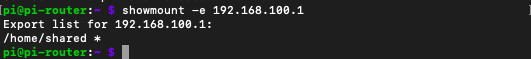
\includegraphics[width=\textwidth]{images/showmount-router.png}
    
    \item You can also test the command from a different cluster node, which should yield the same results:

    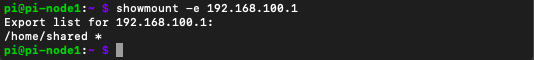
\includegraphics[width=\textwidth]{images/showmount-nonrouter.png}
\end{itemize}
\subsection{Mount shared directory on non-router nodes}

These steps will make the \texttt{/home/shared} directory on the router node available from another cluster node. This will need to be completed on each non-router node.

\begin{itemize}
    \item SSH into the non-router node.
    
    \item Run the following commands on the non-router node:
\begin{verbatim}
# install the NFS client software
sudo apt install nfs-common

# create a directory on which to mount the shared directory
sudo mkdir /home/shared

# allow any user to read, write, and execute the shared files
sudo chmod 777 /home/shared
\end{verbatim}
    
    \item Run \texttt{sudo nano /etc/fstab} to open the file systems table for editing.
    
    \item At the end of the file, add the following on a single line (it's broken up into two lines here to fit the page; use a space instead of a new line):
\begin{verbatim}
192.168.100.1:/home/shared /home/shared nfs 
    rw,hard,intr,noauto,x-systemd.automount 0 0
\end{verbatim}    

    \item Save and close the file.
    
    \item Run \texttt{sudo reboot} and reconnect after the node reboots. When it does, it should have automatically mounted the shared directory that was exported from the router node.
    
    \item To test that the shared directory is working as expected, run \texttt{touch /home/shared/ping} from the non-router node to write an empty file to the shared directory. 
    
    \item On the router node, run \texttt{ls /home/shared} to check that the empty file has appeared there as well. 
\end{itemize}

\section{"Hello World" in MPI}

In this section, you will run a simple program on the cluster using MPI's C interface. The program will be written on the router node in the shared directory created in Section \ref{section/shared-directory}, where it will be visible to all other nodes.

\begin{itemize}
    \item SSH into the router node. The commands in this section will be run on the router node.

    \item Run \texttt{which mpicc} to verify the presence of the MPI C compiler (it should have been installed with MPICH and added to the system path in a previous section). If \texttt{mpicc} is correctly installed, the \texttt{which} command will print its location in the file system.
    
    \item Run the following commands to prepare for writing the Hello World program:
\begin{verbatim}
# create a directory for the program's files
mkdir /home/shared/helloworld

# move to the created directory
cd /home/shared/helloworld

# copy the previously used hostfile into this directory
cp ~/hpl-2.3/bin/rpi/hostfile-all.txt .

# start editing the program source code
nano helloworld.c
\end{verbatim}

    \item Write the following program to \texttt{helloworld.c}:

\begin{verbatim}
#include <mpi.h>
#include <stdio.h>

int main(int argc, char** argv) {
  int process_rank, number_of_processes, hostname_length;
  char hostname[MPI_MAX_PROCESSOR_NAME];

  MPI_Init(&argc, &argv);
  MPI_Comm_size(MPI_COMM_WORLD, &number_of_processes);
  MPI_Comm_rank(MPI_COMM_WORLD, &process_rank);

  MPI_Get_processor_name(hostname, &hostname_length);

  printf("Hello world from process %d of %d on node %s\n", 
    process_rank, number_of_processes, hostname);

  MPI_Finalize();
  return 0;
}
\end{verbatim}

\item Run the command \texttt{mpicc helloworld.c -o helloworld} to compile the program into the executable \texttt{helloworld}.

\item Use \texttt{mpiexec} to run the program with various numbers of processes as follows:

\begin{verbatim}
# by default, mpiexec uses 1 process on the current node
mpiexec ./helloworld

# use the -n argument to assign different numbers of processes:
mpiexec -n 3 ./helloworld
mpiexec -n 12 ./helloworld

# use the -hostfile argument to assign processes on the other cluster nodes:
mpiexec -n 3 -hostfile hostfile-all.txt ./helloworld
mpiexec -n 12 -hostfile hostfile-all.txt ./helloworld
\end{verbatim}

\item The following screenshot shows the expected output when the program is run using 12 processes on the 3-node cluster. 

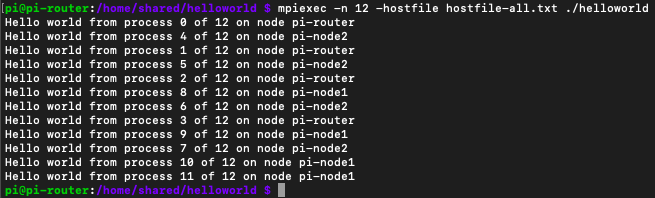
\includegraphics[width=\textwidth]{images/helloworld-output.png}

\textbf{Note:} By default, \texttt{mpiexec} assigns processes to the nodes listed in the hostfile in a round-robin way. That is, one process is assigned to each listed node in order until the required number of processes are assigned, looping through the file if necessary. This is reflected above, where each node is assigned 4 processes.

\item The Hello World program uses several key features of the MPI interface:
    \begin{itemize}
        \item \texttt{MPI\_Init} and \texttt{MPI\_Finalize} must be the first and last MPI calls in any program using MPI. These functions are used to create and destroy the MPI environment, so all MPI usage must occur between their calls.
        
        \item \texttt{MPI\_COMM\_WORLD} is an example of an MPI \emph{communicator}. Each communicator refers to a group of processes, and two different processes can only communicate if they share a communicator. In this case, \texttt{MPI\_COMM\_WORLD} is the default communicator that contains every allocated process.
        
        \item \texttt{MPI\_Comm\_size} determines the number of processes belonging to the communicator passed as an argument.
        
        \item Each communicator maintains a list of processes belonging to it, and the \emph{rank} of a process is its position in that list. \texttt{MPI\_Comm\_rank} determines the rank of the caller's process in the communicator. 
        
        \item \texttt{MPI\_Get\_processor\_name} determines the name of the caller's processor. This can mean different things on different systems, but on the Raspberry Pi cluster it will be the hostname of the caller's node.
    \end{itemize}
\end{itemize}

\section{Prime counting}

In this section we will write a program that counts how many prime numbers there are below $10,000,000$. The program will use a very naive method known as \emph{trial division}, which decides if the number $n$ is prime by checking if $n$ is divisible by any of the numbers between $2$ and $\sqrt{n}$ (if it isn't, then $n$ is prime). The benefit of this method, however, is that it is straightforward to split up the work between any number of parallel processes without needing any interprocess communication.

\begin{itemize}
    \item The commands in this section will once again be run on the router node.
    
    \item Run the following commands to prepare for writing the prime counting program:
\begin{verbatim}
mkdir /home/shared/primes
cd /home/shared/primes
cp ~/hpl-2.3/bin/rpi/hostfile-all.txt .
\end{verbatim}

\item Run \texttt{nano primes.c} and enter the program given in Figure \ref{code:primes}.

\begin{figure}
\begin{Verbatim}[frame=single]
#include <stdio.h>
#include <math.h>
#include <mpi.h>

#define UPPER_LIMIT 10000000

int is_prime(int number) {
  if (number < 2) return 0;

  for (int i = 2; i <= sqrt((double)number); i++) {
    if (number % i == 0) return 0;
  }

  return 1;
}

int main(int argc, char** argv) {
  int rank, process_count;

  MPI_Init(&argc, &argv);
  MPI_Comm_size(MPI_COMM_WORLD, &process_count);
  MPI_Comm_rank(MPI_COMM_WORLD, &rank);

  int primes_found = 0;
  int a = rank + 1;
  int k = process_count + 1;
  for (int n = a; n <= UPPER_LIMIT; n += k) {
    if (is_prime(n) == 1) ++primes_found;
  }

  printf("process %d found %d primes\n", rank, primes_found);

  int primes_found_total, primes_found_max, primes_found_min;
  MPI_Reduce(&primes_found, &primes_found_total, 1, MPI_INT,
	     MPI_SUM, 0, MPI_COMM_WORLD);
  MPI_Reduce(&primes_found, &primes_found_max, 1, MPI_INT,
	     MPI_MAX, 0, MPI_COMM_WORLD);
  MPI_Reduce(&primes_found, &primes_found_min, 1, MPI_INT,
	     MPI_MIN, 0, MPI_COMM_WORLD);

  if (rank == 0) {
    primes_found_total += is_prime(k);
    printf("found %d primes less than or equal to %d\n",
	   primes_found_total, UPPER_LIMIT);
    printf("max found by one process = %d\n, primes_found_max);
    printf("min found by one process = %d\n, primes_found_min);
  }

  MPI_Finalize();
  return 0;
}
\end{Verbatim}
    \caption{\texttt{primes.c} code listing}
    \label{code:primes}
\end{figure}

\item Run the following command to compile the program:
\begin{verbatim}
mpicc ./primes.c -o primes -lm
\end{verbatim}

\textbf{Note:} The argument \texttt{-lm} is required to link the math library that implements the \texttt{sqrt} function.

\item Run the following command to execute the program on the cluster with 12 processes:
\begin{verbatim}
time mpiexec -n 12 -hostfile hostfile-all.txt ./primes
\end{verbatim}

\textbf{Note:} The \texttt{time} command prefix times the following \texttt{mpiexec} command and prints the result. This is a simple way to time any command that doesn't have a built-in timer. For multithreaded programs, the \texttt{real}-time measurement is more useful than the \texttt{user} and \texttt{system} measurements.

\item Modify the previous command to time the program's execution when $4$, $6$, and $10$ processes are used instead of $12$. Verify that your observed execution times are similar to Table \ref{tab:primes-time}.

\textbf{Note:} The issue in Assignment 1 (where an incorrect number of processes were used by MPI) does not occur here. The \texttt{-n} argument to \texttt{mpiexec} seems to correctly spawn the desired number of processes across the cluster.

\begin{table}[]
\centering
\begin{tabular}{c|c}
\hline
\textbf{\begin{tabular}[c]{@{}c@{}}Processes\\ used\end{tabular}} & \textbf{\begin{tabular}[c]{@{}c@{}}Real-time\\ duration (s)\end{tabular}} \\ \hline
4                                                                 & 21.754                                                                    \\
6                                                                 & 14.681                                                                    \\
10                                                                & 9.023                                                                     \\
12                                                                & 7.900                                                                     \\ \hline
\end{tabular}
\caption{Sample real-time durations of the prime-counting program.}
\label{tab:primes-time}
\end{table}

\textbf{Note:} Each process searches for primes among the numbers of the form $(r + 1) + k(p + 1)$, where $r$ is the process' rank and $p$ is the total number of processes. This works well when $p + 1$ is itself a prime number, in which case the primes will roughly be evenly distributed between processes (by Dirichlet's prime number theorem). When $p + 1$ is not prime, however, then the workload will be highly imbalanced between processes (with some processes finishing almost immediately) and the observed execution duration will go up significantly.

\item The only new feature of MPI used by the prime-counting program is \texttt{MPI\_Reduce}. Generally speaking, \texttt{MPI\_Reduce} is passed a value from each process in a communicator and \emph{reduces} those values into a single result via an operation that's also specified in the call.

For example, given the call:
\begin{verbatim}
MPI_Reduce(&primes_found, &primes_found_total, 1,
           MPI_INT, MPI_SUM, 0, MPI_COMM_WORLD);
\end{verbatim}
    \begin{itemize}
        \item The call will receive the value of \texttt{primes\_found} (which is of type \texttt{MPI\_INT}) from each process in the \texttt{MPI\_COMM\_WORLD} communicator.
        \item  It will reduce those values via the \texttt{MPI\_SUM} operation, which adds the values together as it receives them.
        \item The resulting sum of all values will be stored in the variable \texttt{primes\_found\_total}.
        \item Only the process with rank $0$ (specified in the second-to-last argument) will receive the result. The process that receives the result is also known as the \emph{root} process.
        \item \texttt{MPI\_Reduce} is \emph{blocking}, which means that MPI will pause processes that reach the reduce call until every process in the communicator has reached that point in the program. This ensures that the final sum won't be printed by the root process until each process has contributed its \texttt{primes\_found} value to the total sum.
    \end{itemize}

\item Similarly, the second call to \texttt{MPI\_Reduce} uses the \texttt{MPI\_MAX} operation, which stores the maximum of all \texttt{primes\_found} values into \texttt{primes\_found\_max}. The third call uses the \texttt{MPI\_MIN} operation, which stores the minimum value into \texttt{primes\_found\_min}.
\end{itemize}

\section{Round-robin scheduler}
This section will implement a minimal round-robin scheduler using MPI. In this context, \emph{round-robin} means using processes in a circular order, returning to use the first process after the last process has been used.

Given $n$ processes, our program will use the rank $0$ process as the \emph{scheduler} process and the remaining $n-1$ processes (with ranks $1$ through $n - 1$) as \emph{server} processes. The scheduler will pass messages (represented by increasing numbers) to the servers in round-robin order, as shown in the following screenshot:
\\~\\
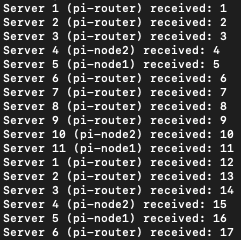
\includegraphics[scale=0.5]{images/roundrobin-output.png}

\begin{itemize}
\item Create the \texttt{roundrobin} directory for this section's program in the \texttt{/home/shared} directory as in the previous sections.

\item Copy the \texttt{hostfile-all.txt} hostfile to the newly created \texttt{roundrobin} directory.

\item Begin editing the \texttt{roundrobin.c} file inside the \texttt{roundrobin} directory and write the program given in Figure \ref{code:roundrobin}.

\item Run the following command to compile the program:
\begin{verbatim}
mpicc ./roundrobin.c -o roundrobin
\end{verbatim}

\item Run the following command to execute the program:
\begin{verbatim}
mpiexec -n 12 -hostfile hostfile-all.txt ./roundrobin
\end{verbatim}

\begin{figure}
\begin{Verbatim}[frame=single]
#include <stdio.h>
#include <unistd.h>
#include <mpi.h>

void run_scheduler_process(int process_count) {
  int next_server = 1, next_data = 1;
  while (1) {
    MPI_Send(&next_data, 1, MPI_INT, next_server, 
             0, MPI_COMM_WORLD);
    next_data++;
    next_server++;
    if (next_server == process_count) next_server = 1;
    usleep(300000);
  }
}

void run_server_process(int rank, char* hostname) {
  int data, request_complete;
  MPI_Request request;
  while (1) {
    MPI_Irecv(&data, 1, MPI_INT, 0, 0, MPI_COMM_WORLD, &request);
    request_complete = 0;
    while (!request_complete) {
      MPI_Test(&request, &request_complete, MPI_STATUS_IGNORE);
      usleep(300000);
    }
    printf("Server %d received: %d\n", rank, hostname, data);
  }
}

int main(int argc, char** argv) {
  int rank, process_count, hostname_length;
  char hostname[MPI_MAX_PROCESSOR_NAME];

  MPI_Init(&argc, &argv);
  MPI_Comm_size(MPI_COMM_WORLD, &process_count);
  MPI_Comm_rank(MPI_COMM_WORLD, &rank);
  MPI_Get_processor_name(hostname, &hostname_length);

  if (rank == 0) {
    printf("Starting scheduler (rank 0) on %s\n", hostname);
    run_scheduler_process(process_count);
  } else {
    printf("Starting server (rank %d) on %s\n", rank, hostname);
    run_server_process(rank, hostname);
  }

  MPI_Finalize();
  return 0;
}
\end{Verbatim}
    \caption{\texttt{roundrobin.c} code listing}
    \label{code:roundrobin}
\end{figure}

\textbf{Note:} The shortcut Control+C can be used to exit the program while it's still running and regain control of the terminal. This shortcut isn't specific to this program and should interrupt any program running in a terminal.

\item This program introduces the concept of \emph{message passing} in MPI, after which MPI is named.
\begin{itemize}
        \item The scheduler process sends a message with the call:
\begin{verbatim}
    MPI_Send(&next_data, 1, MPI_INT, next_server, 0, MPI_COMM_WORLD);\end{verbatim}
    This sends the integer variable \texttt{next\_data} to the process with rank \texttt{next\_server}. \texttt{MPI\_Send} is \emph{blocking}, which means that the scheduler process halts execution until the message is received by the targeted server process.
    
    \item A server process receives a message with the call:
\begin{verbatim}
    MPI_Irecv(&data, 1, MPI_INT, 0, 0, MPI_COMM_WORLD, &request);\end{verbatim}
    This receives the integer sent by the process of rank $0$ (the scheduler) and stores it in the variable \texttt{data}. \texttt{MPI\_Irecv} is \emph{non-blocking}, which means that the server process will continue execution after the call, and that the message will be received and stored in \texttt{data} asynchronously (at some unknown future time). The status of the message is maintained in \texttt{request}, and will reflect when the data has been received.
    
    \item Since \texttt{MPI\_Irecv} is asynchronous, the caller needs to test the \texttt{request} variable to know when the message has been received. The following \texttt{while} loop accomplishes this using \texttt{MPI\_Test}:
\begin{verbatim}
    request_complete = 0;
    while(!request_complete) {
        MPI_Test(&request, &request_complete, MPI_STATUS_IGNORE);
        usleep(300000);
    }\end{verbatim}
    The \texttt{MPI\_Test} call checks if \texttt{request} refers to a completed message, and if so will set \texttt{request\_complete} to $1$, which will lead to the loop being exited.
    
    \item Using the blocking receive function \texttt{MPI\_Recv} instead of \texttt{MPI\_Irecv} is undesirable here since the messages are sent to the server relatively infrequently. A blocking call uses a high amount of CPU while waiting, which would be inefficient given the sparsity of the messages.
    \end{itemize}

\end{itemize}

\section{Broadcast benchmark}

This section is adapted from the \texttt{MPI\_Bcast} article of Resource \ref{resource:mpitutorial}.

The previous section analyzed a program where messages were sent from one process to another. In some cases, however, it is desirable for data to be shared throughout a larger group of processes (in MPI, processes are grouped together into \emph{communicators}).
The MPI function \texttt{MPI\_Bcast} exists for this purpose: to efficiently send a message from one root process in a communicator to the rest.

Of course, this functionality could be duplicated naively by repeatedly calling \texttt{MPI\_Send} from the root process, targeting each other nonroot process in the communicator. The programs in this section will compare repeated calls of \texttt{MPI\_Send} to using \texttt{MPI\_Bcast}, and will show that \texttt{MPI\_Bcast} significantly outperforms the naive method even in a relatively small communicator. 

To explain the gap in performance between \texttt{MPI\_Send} and \texttt{MPI\_Bcast}, consider a loop such as the following, which naively sends data from the root process of rank 0 to the $n$ nonroot processes of ranks $1$ through $n$:
\begin{verbatim}
for (int rank = 1; rank < n; rank++) {
  MPI_Send(&data, 1, MPI_INT, rank, 0, MPI_COMM_WORLD);
}
\end{verbatim}
Before the loop starts, the data is only present on process 0. After one iteration, process 0 sends the data to process 1, so the data is present on those two processes. Thus, in this implementation, process 1 idles for the remainder of the loop while it waits for process 0 to send the data to the remaining processes. 

This is an inefficiency that \texttt{MPI\_Bcast} at least partially alleviates. When using \texttt{MPI\_Bcast}, nonroot processes that have been sent the shared data will continue sending it to other processes that still need it, rather than idling until the end of the loop as in the naive method. This extra functionality is built into \texttt{MPI\_Bcast} automatically, and will be used by MPI when \texttt{MPI\_Bcast} is called on each process in the communicator. This is demonstrated in the \texttt{bcast.c} program in Figure \ref{code:bcast}.

\begin{itemize}
\item Create the \texttt{bcast} directory for this section's program in the \texttt{/home/shared} directory as in the previous sections.

\item Copy the \texttt{hostfile-all.txt} hostfile to the newly created \texttt{bcast} directory.

\item Write the programs given in Figures \ref{code:send} and \ref{code:bcast} into the files \texttt{send.c} and \texttt{bcast.c}, respectively.

\item Use \texttt{mpicc} to compile the two programs into the \texttt{send} and \texttt{bcast} executables.

\item Use \texttt{mpiexec} to execute the two programs using the usual hostfile and 12 processes.

\item Run both programs. The output for \texttt{send} and \texttt{bcast} should look similar to the following screenshots, respectively:

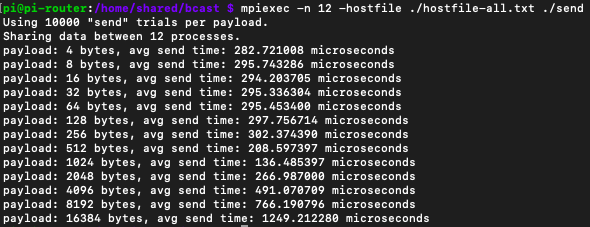
\includegraphics[width=\textwidth]{images/send-output.png}

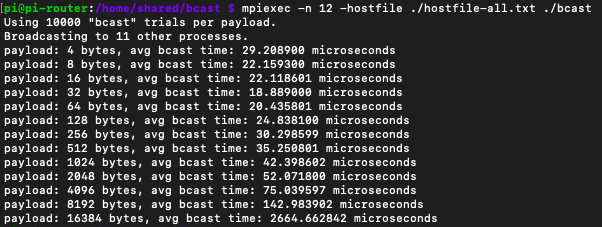
\includegraphics[width=\textwidth]{images/bcast-output.png}

\textbf{Note:} Interestingly, the performance of \texttt{MPI\_Bcast} drops sharply on the largest payload size, doing much worse than \texttt{MPI\_Send}. It's not clear why this might be.
\end{itemize}

\begin{figure}
\begin{Verbatim}[frame=single]
#include <mpi.h>
#include <stdio.h>
#include <time.h>

#define TRIALS 10000
#define COMM MPI_COMM_WORLD

long long get_microsecond_timestamp() {
  struct timespec ts;
  clock_gettime(CLOCK_REALTIME, &ts);
  return (ts.tv_sec) * 1e6 + ts.tv_nsec / 1e3;
}

void run_root_process(int data_size, int world_size) {
  int data[data_size];
  long long start_time = get_microsecond_timestamp();
  for (int trial = 0; trial < TRIALS; trial++) {
    for (int rank = 1; rank < world_size; rank++) {
      MPI_Send(&data, data_size, MPI_INT, rank, 0, COMM);
    }
  }
  long long duration = get_microsecond_timestamp() - start_time;
  float average_duration = (float)duration / TRIALS;
  printf("payload: %d bytes, avg send time: %.6f microseconds\n",
	 sizeof(int) * data_size, average_duration);
}

void run_nonroot_process(int data_size) {
  int data[data_size];
  for (int trial = 0; trial < TRIALS; trial++) {
    MPI_Recv(&data, data_size, MPI_INT, 0, 0, COMM,
	     MPI_STATUS_IGNORE);
  }
}

int main(int argc, char** argv) {
  int rank, world_size;
  MPI_Init(&argc, &argv);
  MPI_Comm_rank(COMM, &rank);
  if (rank == 0) {
    MPI_Comm_size(COMM, &world_size);
    printf("Using %d \"send\" trials per payload.\n", TRIALS);
    printf("Sharing data between %d processes.\n", world_size);
  }
  for (int size = 1; size < (2 << 12); size *= 2) {
    if (rank == 0) run_root_process(size, world_size);
    else run_nonroot_process(size);
  }
  MPI_Finalize();
  return 0;
}
\end{Verbatim}
    \caption{\texttt{send.c} code listing}
    \label{code:send}
\end{figure}

\begin{figure}
\begin{Verbatim}[frame=single]
#include <mpi.h>
#include <stdio.h>
#include <time.h>

#define TRIALS 10000
#define COMM MPI_COMM_WORLD

long long get_microsecond_timestamp() {
  struct timespec ts;
  clock_gettime(CLOCK_REALTIME, &ts);
  return (ts.tv_sec) * 1e6 + ts.tv_nsec / 1e3;
}

void run_root_process(int data_size) {
  int data[data_size];
  long long start_time = get_microsecond_timestamp();
  for (int trial = 0; trial < TRIALS; trial++) {
    MPI_Bcast(&data, data_size, MPI_INT, 0, COMM);
  }
  long long duration = get_microsecond_timestamp() - start_time;
  float average_duration = (float)duration / TRIALS;
  printf("payload: %d bytes, avg bcast time: %.6f microseconds\n",
	 sizeof(int) * data_size, average_duration);
}

void run_nonroot_process(int data_size) {
  int data[data_size];
  for (int trial = 0; trial < TRIALS; trial++) {
    MPI_Bcast(&data, data_size, MPI_INT, 0, COMM);
  }
}

int main(int argc, char** argv) {
  int rank, world_size;
  MPI_Init(&argc, &argv);
  MPI_Comm_rank(COMM, &rank);
  if (rank == 0) {
    MPI_Comm_size(COMM, &world_size);
    printf("Using %d \"bcast\" trials per payload.\n", TRIALS);
    printf("Broadcasting to %d other processes.\n",
	   world_size - 1);
  }
  for (int size = 1; size < (2 << 12); size *= 2) {
    if (rank == 0) run_root_process(size);
    else run_nonroot_process(size);
  }
  MPI_Finalize();
  return 0;
}
\end{Verbatim}
    \caption{\texttt{bcast.c} code listing}
    \label{code:bcast}
\end{figure}

\section{Resources}

\begin{enumerate}

\item Documentation for the MPICH C language API:

\url{https://www.mpich.org/static/docs/latest/}

\item Documentation for OpenMPI, another implementation of MPI:

\url{https://www.open-mpi.org/doc/current/}

\item \label{resource:mpitutorial} Articles explaining some introductory concepts of MPI programming:

\url{https://mpitutorial.com/tutorials/}
    
\end{enumerate}


\end{document}
